\chapter{Experiment and Results}

\section{Experiment}
To measure the accuracy of the developed system, the \ac{ROS} setup similar as described in \autoref{subsec:tracking} was used. The \ac{EKF} works in the camera coordinate systems with approximately $80\mathit{Hz}$. To eases the whole handling, the experiments were recorded with rosbag and then afterwards off-line evaluated with a separate python script.

To have a ground truth to compare with, the 3D coordinates of the tracked object measured by a motion capture system (VICON) were additionally recorded.

For the comparison between the accuracy of the \ac{UWB} system and the one of the \ac{EKF}, both systems were compared with the mentioned ground truth by the root mean squared error $$\textit{rmse} = \frac{1}{\#\text{ of elements}} \sum_i \sqrt{(x_{m,i} - x_{V,i})^2 + (y_{m,i} - y_{V,i})^2 + (z_{m,i} - z_{V,i})^2}$$
and by the root mean squared error of only the $x$ and $y$ axis
$$\textit{rmse}_{xy} = \frac{1}{\#\text{ of elements}} \sum_i \sqrt{(x_{m,i} - x_{V,i})^2 + (y_{m,i} - y_{V,i})^2}$$

where the subfix $m$ stands for measurement and represents coordinates which either come from the \ac{UWB} system or from the \ac{EKF}. The subfix $V$ on the other hand stands for VICON which is the ground truth in this experiment. 

\section{Results}
On several recorded experiments, the $\textit{rmse}$ and the $\textit{rmse}_{xy}$ of the \ac{EKF} was significantly lower compared to the $\textit{rmse}$ and the $\textit{rmse}_{xy}$ of the \ac{UWB}. The results of some experiments are listed in \autoref{tab:results}. A 3D plot of the measured coordinates by the VICON system (ground truth), the \ac{UWB} system and the coordinates fused by the \ac{EKF} from a data set is shown in \autoref{fig:evaluation}.

\begin{table}[ht!]
\begin{center}
\begin{tabular}{c|c|c|c|c}
	Experiment number & $\textit{rmse}$ of \ac{UWB} & $\textit{rmse}$ of \ac{EKF} & $\textit{rmse}_{xy}$ of \ac{UWB} & $\textit{rmse}_{xy}$ of \ac{EKF}\\ 
	\hline 
	1 & 0.0753 & 0.0278 & 0.0705 & 0.0171 \\
	2 & 0.0732 & 0.0290 & 0.0681 & 0.0169 \\ 
	%\hline 
\end{tabular}
\end{center}
\caption{Table with listed $\textit{rmse}$ and $\textit{rmse}_{xy}$ of the \ac{UWB} system and the \ac{EKF} for the different experiments.}
\label{tab:results}
\end{table}

\begin{figure}[ht!]\centering
	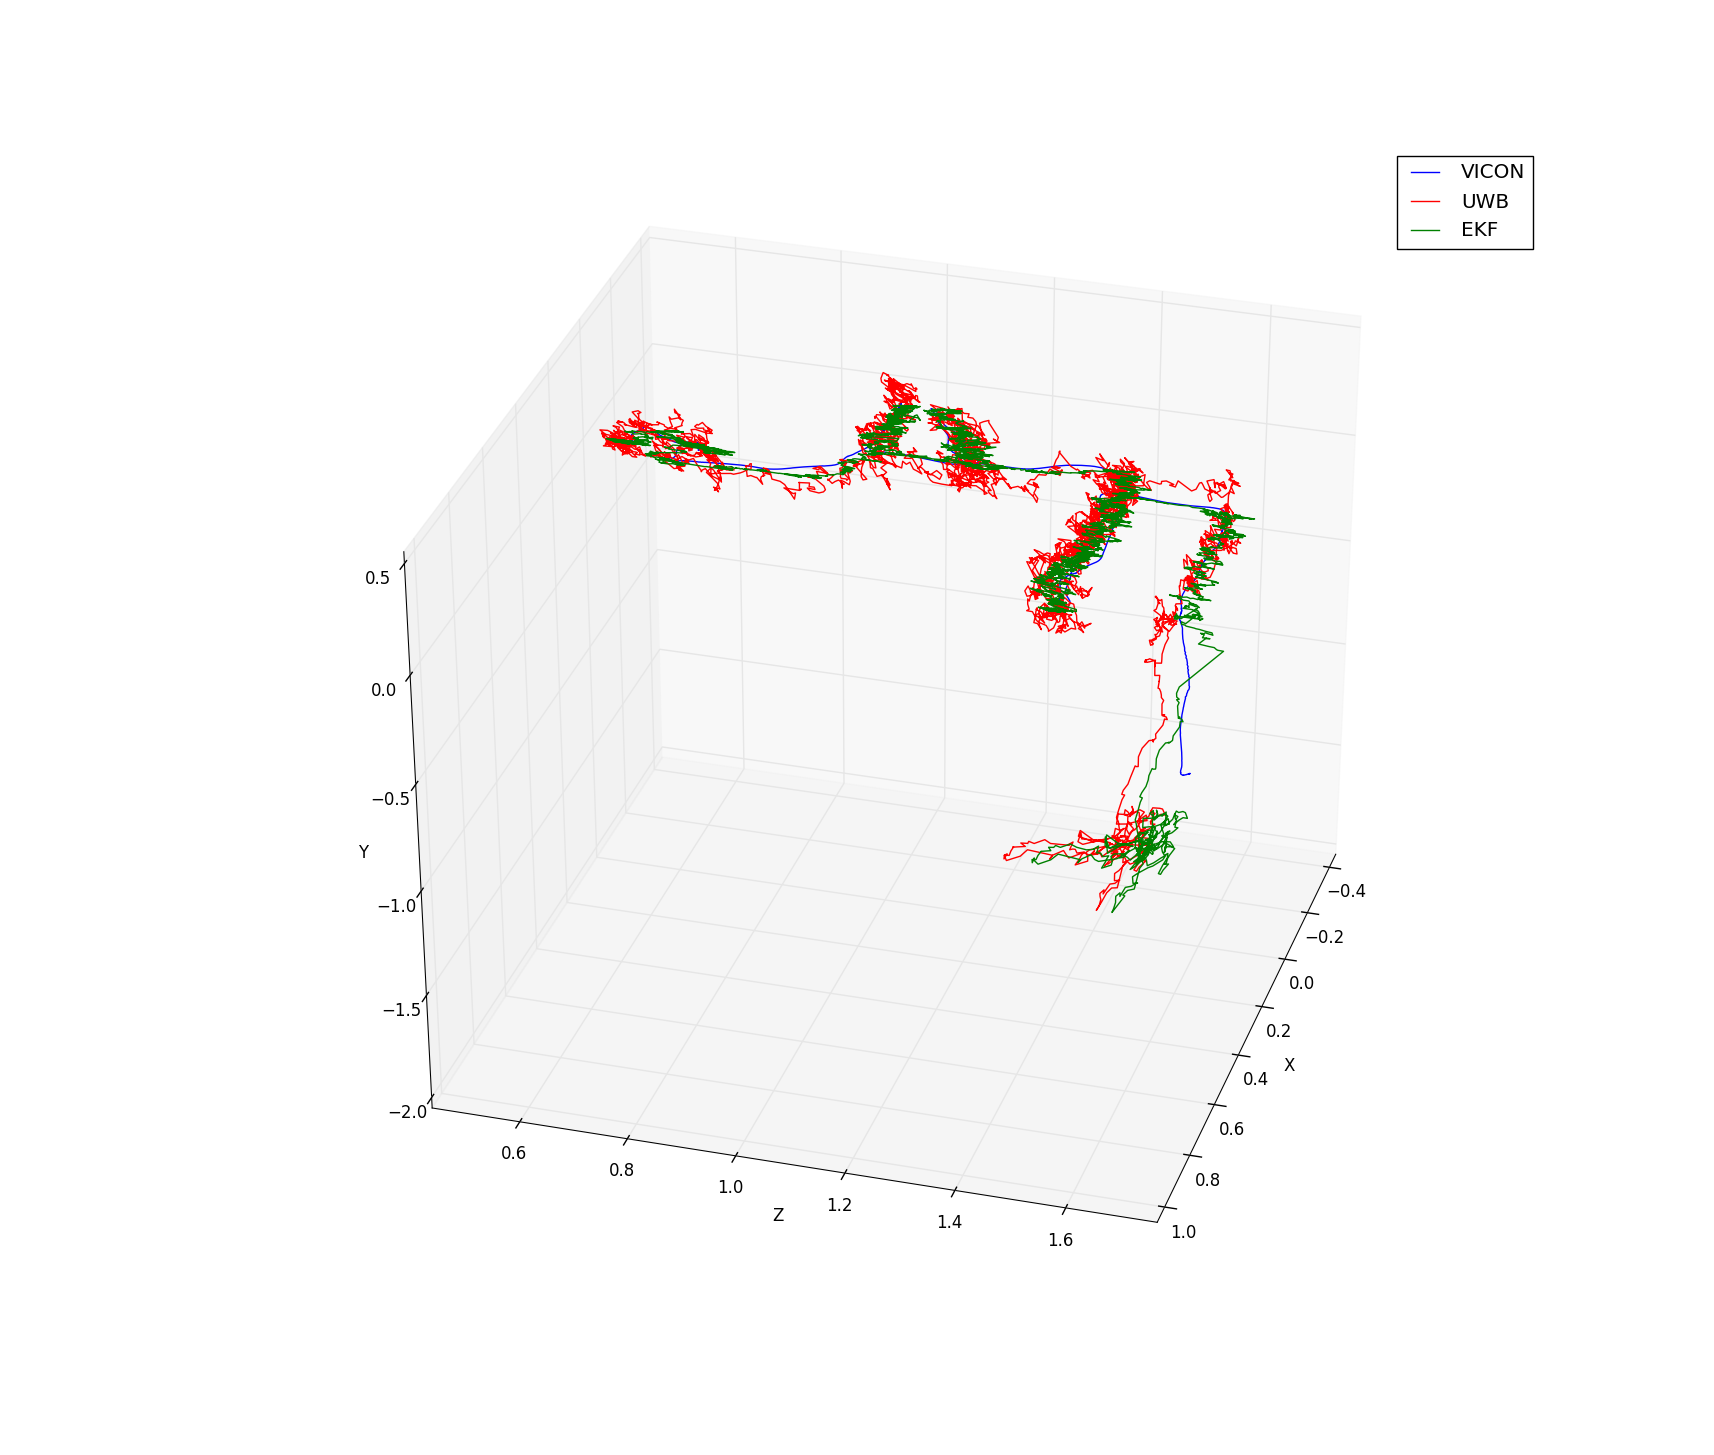
\includegraphics[width=1.0\textwidth]{figures/evaluation}
	\caption{3D pot of the measured coordinate points by the \ac{UWB} system (red), the measured point by the VICON system (blue) and the fused positions (green)}\label{fig:evaluation}
\end{figure}
